\subsection{Builder Marketplace}
The Builder Marketplace is a next-generation ecosystem designed to streamline cross-chain communication for decentralized applications (dApps) by leveraging a network of modular solvers. These solvers integrate existing blockchain protocols across multiple chains, ensuring seamless interoperability and enhanced functionality for dApps. Our approach is unique in that we aggregate existing protocols from all blockchain networks and create modular representations of each dApp within our architecture. These dApp modules encapsulate all relevant information about a given application, enabling official teams to access, manage, and update their modules through a dedicated dashboard, similar to how APIs are managed and deployed on platforms like Postman today.

\begin{figure}[h]
    \centering
    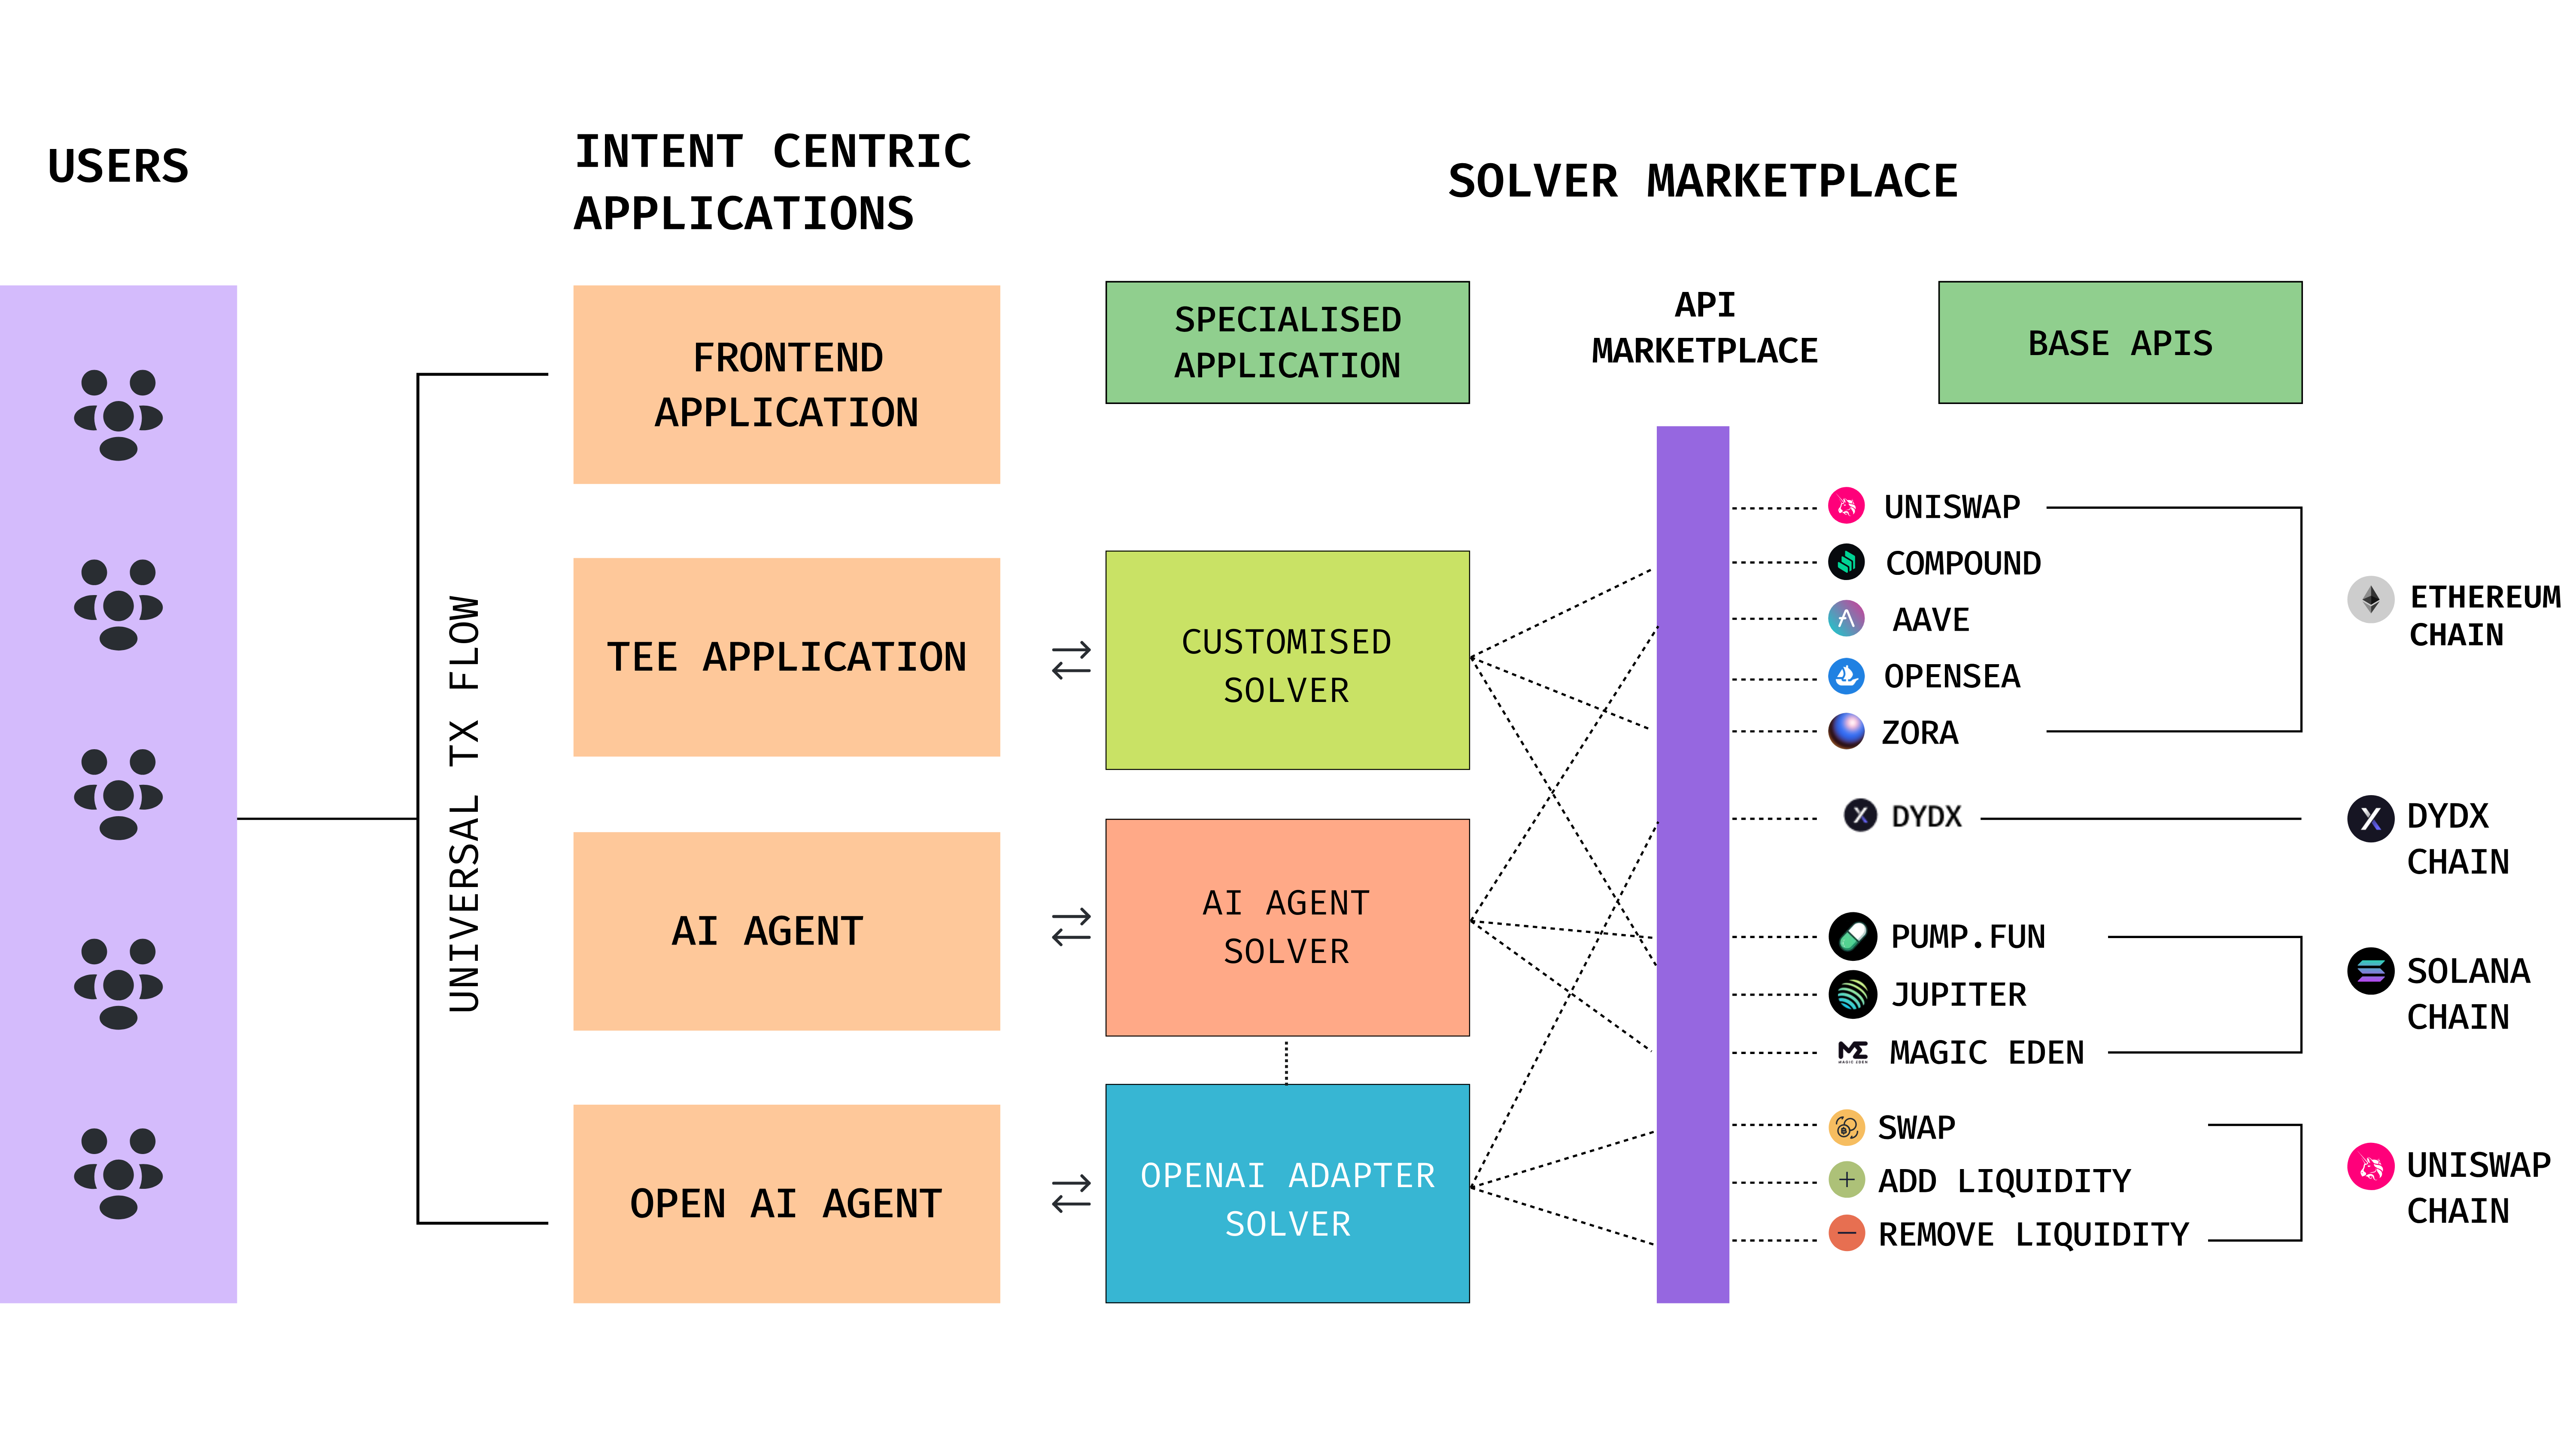
\includegraphics[width=0.9\linewidth]{figure/builder.png}
    \caption{Builder Marketplace Overview}
    \label{fig:builder}
\end{figure}

Beyond these dApp modules, developers can build customized solvers by merging functionalities from multiple modules. This allows for flexible and composable solutions, ensuring seamless cross-communication between solvers while optimizing execution paths. The Builder Marketplace supports universal transaction flows, catering to intent-centric applications, AI agents, and direct API calls from frontend applications. In addition, these specialized and base solvers feature dedicated interfaces, which can be used by intent-centric protocols and AI agents, further enhancing the interoperability, efficiency, and scalability of decentralized applications. By providing a structured yet adaptable framework, the Builder Marketplace serves as a powerful foundation for the next wave of blockchain-powered innovations.

By focusing on solver-driven execution, cross-chain interoperability, and a modular architecture, the Builder Marketplace empowers developers to create highly efficient and scalable solutions for decentralized applications. This ecosystem bridges the gap between disparate blockchain networks, offering a unified platform for seamless transaction execution and inter-chain communication.

\begin{figure}[h]
    \centering
    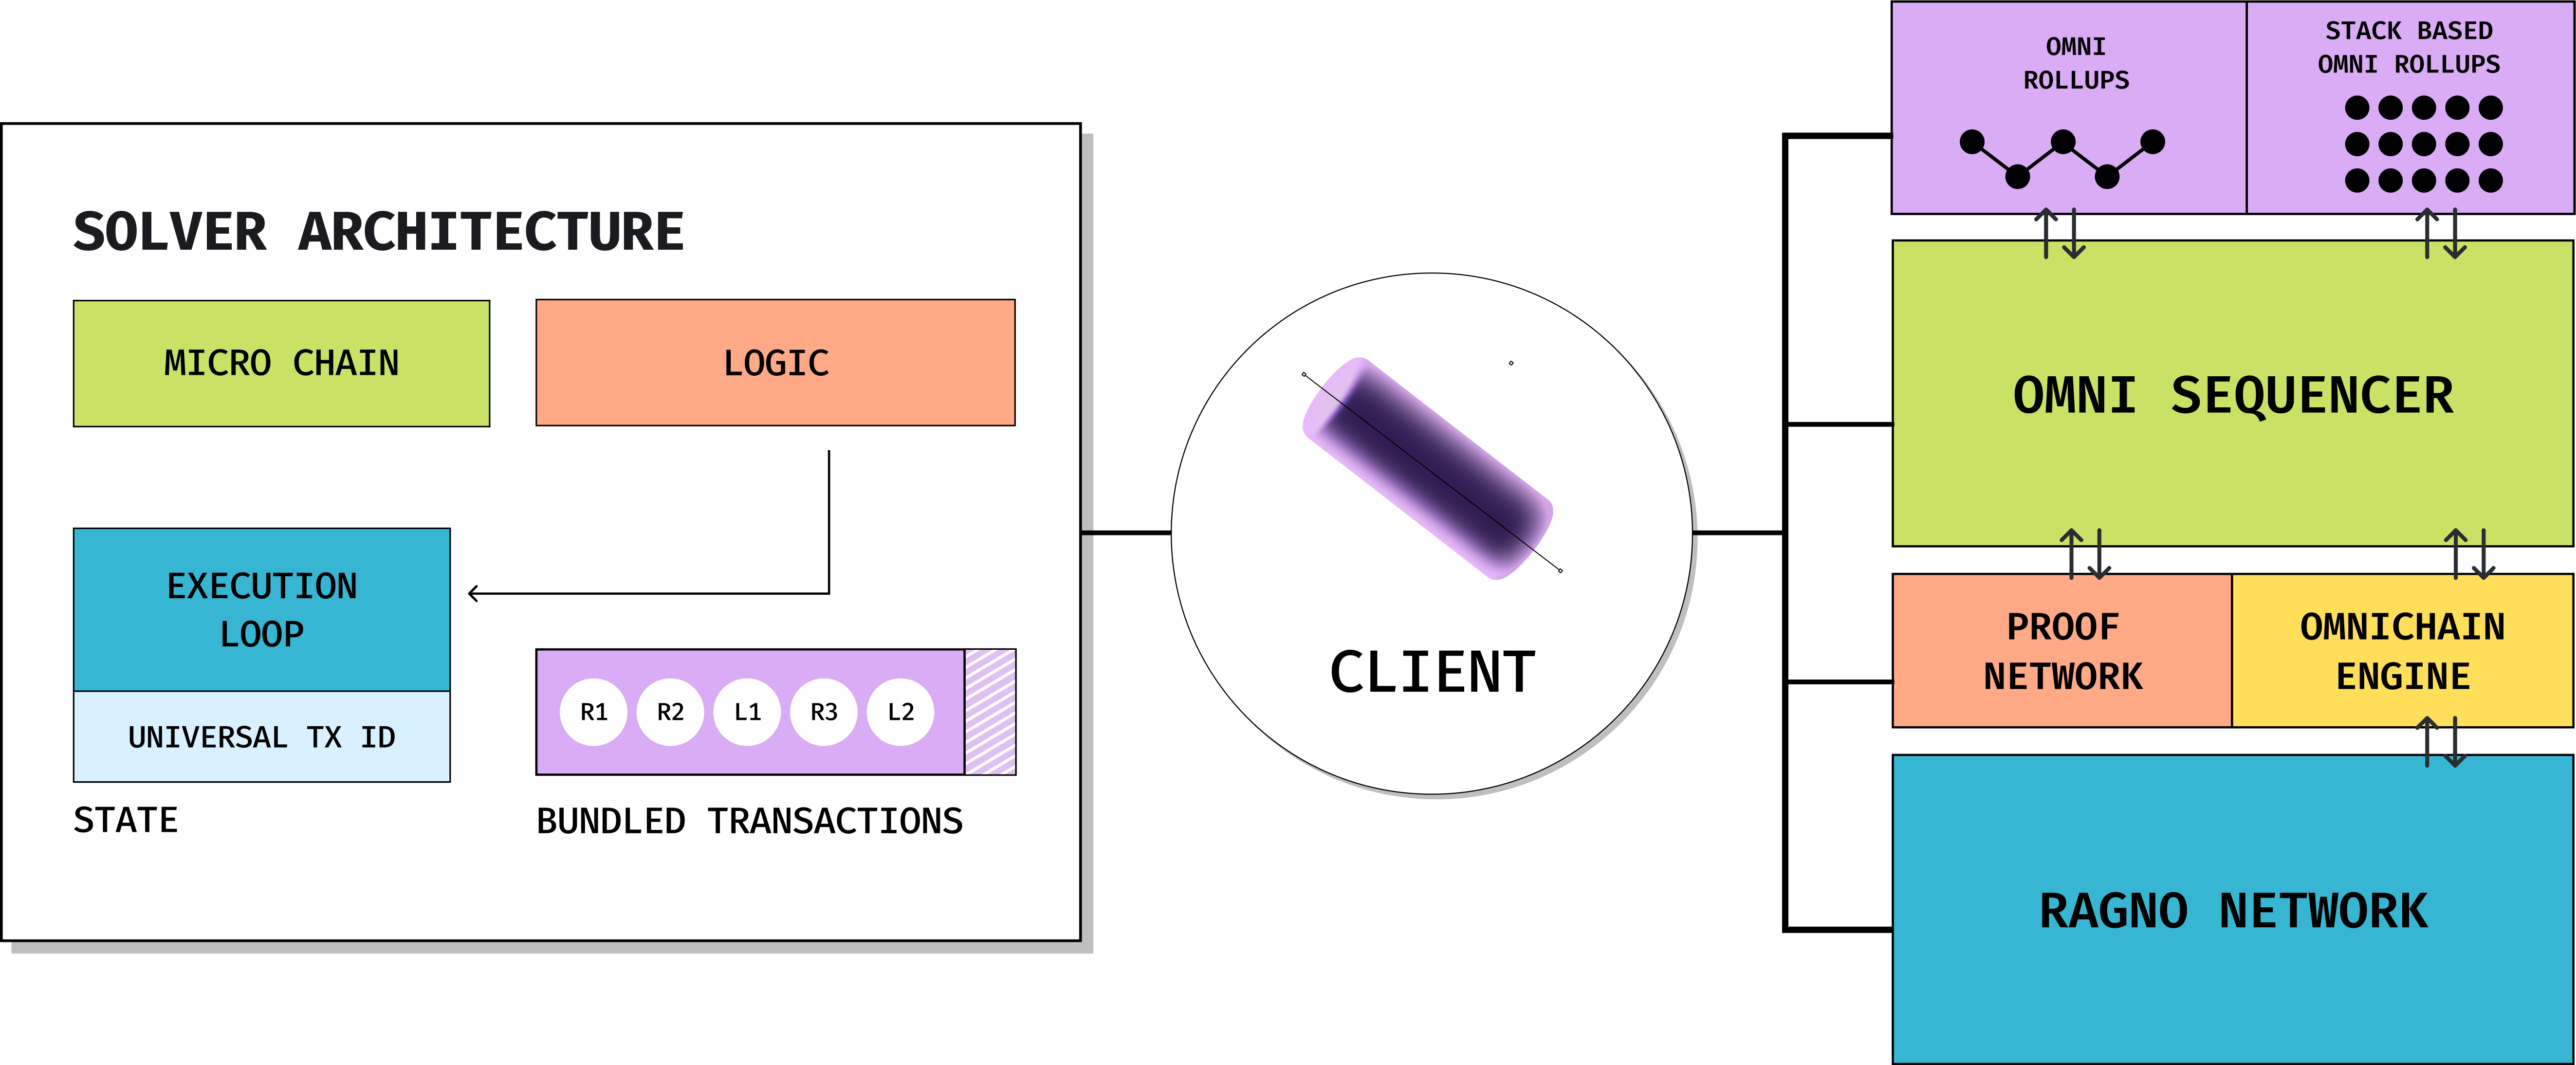
\includegraphics[width=0.9\linewidth]{figure/solver.png}
    \caption{Solver Illlustration}
    \label{fig:solver}
\end{figure}

\subsubsection{Solver Network}
The Solver Network operates as a decentralized network of solvers, each running its own Linera microchain~\cite{linera} to support various base API services. Each microchain contains critical components such as Rust-based logic for operations, addresses on different supported blockchain networks, and an information module for various base APIs. This modular architecture enables solvers to independently process transactions while maintaining interoperability within the broader solver ecosystem.

When a transaction is received, a solver performs rigorous verification processes. Validity checks ensure that input dependencies and execution feasibility are met, while authenticity is validated through user signatures. Once verified, the solver executes the transaction autonomously or collaborates with other solvers if additional resources or interactions are required to optimally fulfill the user intent.

Each solver is equipped with a dedicated client that facilitates integration with the Omni Sequencer, Prover Network, and Omnichain Engine. For omni-rollup transactions, the solver bundles transactions and forwards them to the Omni Sequencer, which orders them and dispatches them to the appropriate rollup for execution. The client continuously monitors these transactions, providing preconfirmation and confirmation updates to ensure reliable tracking and visibility of execution status.

For direct Layer 1 (L1) settlements using solver-owned addresses, solvers interact with Hermes validators for execution. To secure these transactions, the Threshold Signature Scheme (TSS) is used. Each solver’s client generates secret shares for its addresses on different blockchains, retaining one share while distributing the remaining shares among Hermes validators. This distribution is structured so that the solver's participation in the signing is essential to generate a valid transaction signature. Depending on the transaction type, the client interacts with the Omni Sequencer for rollup transactions or directly executes transactions on L1 chains via Hermes validator sets.

Direct settlement through solvers significantly enhances cross-chain transaction efficiency by reducing reliance on intermediary networks and ensuring streamlined execution. Using decentralized computation, advanced cryptographic mechanisms, and a modular execution environment, the Solver Network provides a robust foundation for executing user intents in a highly efficient and secure manner.

\subsubsection{Transaction Flow}
The transaction flow in the Builder Marketplace is designed to accommodate multiple types of transactions, ensuring seamless execution from the initiation to the final settlement. The different types of transaction include intent-centric transactions, AI-driven transactions, and direct API call transactions. Below is a breakdown of the transaction flow:
\begin{itemize}
    \item \textbf{Transaction Initiation}:

    Transactions can be initiated through intent-centric applications, AI agents, or direct API calls from front-end applications. Once a transaction request is submitted, the solver network analyzes it and determines the most efficient execution route.

    \item \textbf{Solver Selection and Processing}:

    The appropriate solver or group of solvers is chosen based on the characteristics of the transaction. They validate the transaction by verifying the input dependencies and feasibility. Cryptographic signatures are used to ensure authenticity.

    \item \textbf{Cross-Chain Communication and Execution}:

    For cross-chain transactions, solvers communicate via the microchain structure, utilizing integrated blockchain protocols for efficient execution. When omni-rollup handling is required, solvers bundle the transaction and forward it to the Omni Sequencer, which organizes and submits it to the appropriate rollup for execution.

    \item \textbf{Finalization and Settlement}:

    For omni-rollup transactions, the solver network monitors transaction progress, providing pre-confirmation and final confirmation updates. In the case of direct Layer 1 (L1) settlements, the solver collaborates with Hermes validators to execute the transaction. The final transaction state is then recorded on the relevant blockchain, ensuring both transparency and immutability.
    
    \item \textbf{Confirmation and Feedback}:
    
    Users receive updates on the transaction status in real time through the interface of the solver network. The system is designed to ensure efficient and secure transaction completion, optimizing minimal latency while maintaining maximum security.
\end{itemize}

    
This structured transaction flow ensures that the Builder Marketplace efficiently handles a diverse range of transactions while maintaining high performance, security, and scalability.